\documentclass[../main.tex]{subfiles}
\begin{document}
\chapter{Background}\label{back:chap}
\section{Sequential Decision Making}

\emph{Sequential Decision Making (SDM)} is the field studying problems and approaches wherein an
artificial agent interacts with an environment in the process of pursuing and eventually achieving
a specific goal~\citep{frankish_cambridge_2014}. In this context, we envision the agent as acting
according to some \emph{policy} $\pi$ which maps states $S$ to actions $A$. States are instantaneous
representations of the environment, descriptions of the environment at a given moment. Actions are
motions and outputs produced by the agent that may affect the state of the environment. We model the
interaction between the agent and the environment as unfolding over discrete time steps. At each
time step, the agent observes the state, consults its policy $\pi$ to select an action, and then
executes that action. In the next time step, the environment responds by transitioning to a new
state, and the loop continues.

What we are gradually formalizing here is the classical \emph{Markov Decision Process (MDP)}
framework~\citep{puterman_markov_2014} for SDM, shown in Figures~\ref{fig:mdp-classic}
and~\ref{fig:mdp-causal}. Aside for states $S$ and actions $A$, an MDP additionally consists of

\begin{itemize}
	\item A \emph{transition function} $P : S \times A \times S \rightarrow [0, 1]$, describing the
	      probability that action $a$ in state $s$ will lead to state $s'$.
	\item A \emph{reward function} $R : S \times A \times S \rightarrow \mathbb{R}$, the immediate reward
	      achieved when transitioning from state $s$ to state $s'$ via action $a$.
\end{itemize}

The agent interacting with the MDP gives rise to a discrete sequence of states, actions and rewards
known as a $trajectory$, indexed by time-steps $t$ and taking the form

\begin{equation*}
	S_0, A_0, R_1, S_1, A_1, R_2, S_2, A_2, \dots, S_t, A_t, R_{t+1}, S_{t+1}, A_{t+1}.
\end{equation*}

We note that the transition function only depends on the current state and action, implying that
current state is independent of all but the previous state. This is the \emph{Markov property}.

The reward function is a proxy of how well the agent is doing in pursuing a specific task.
\emph{Reinforcement Learning (RL)} can then be defined as learning how to act interactively to
maximize expected cumulative reward~\citep{sutton_reinforcement_2018}.

The transition function of the MDP is often unavailable to the agent and must be modeled either
implicitly or explicitly. Similarly, the reward function is often unavailable or underspecified,
making RL impractical to use. What is sometimes available instead, are (close to) expert
demonstrations of the task at hand. \emph{Imitation Learning (IL)} can be defined as the
optimization of a policy $\pi_{\text{IL}}$ such that it behaves similarly to a given expert or set
of experts~\citep{schaal_is_1999}. In our work, we focus on \emph{behavioural cloning
	(BC)}~\citep{michie_cognitive_1990}, reducing our SDM problem to supervised learning.

In general there is no ``one-size-fits-all'' solution to SDM. However, MDPs, while limited in some
ways, provide sufficient flexibility for a variety of approaches.

\begin{figure}[t]
	\centering
	\includegraphics[width=\textwidth]{figures/mdp-classic}
	\caption[The agent-environment loop of a Markov decision process.]{The agent-environment loop of a Markov decision
		process.}
	\label{fig:mdp-classic}
\end{figure}
\afterpage{
	\begin{figure}[t]
		\centering
		\includegraphics[width=\textwidth]{figures/mdp-causal}
		\caption[A Markov decision process visualized as a causal graph.]{A Markov decision process
			visualized as a causal graph.}
		\label{fig:mdp-causal}
	\end{figure}
}


\section{Goal Misgeneralization}

Goal Misgeneralization (GMG) is an empirically observed failure mode of machine learning models,
particularly closely tied to SDM. Two existing definitions exist for the same phenomenon which we
present below for background.

\Citet{langosco_goal_2022} are the first to formally identify the issue of GMG, describing it as
a form of out-of-distribution (OOD) robustness~\citep{arjovsky_out_2020} failure in RL. They
specifically distinguish it from ``capability generalization failures'', where an agent deployed OOD
simply fails to take useful actions. Instead, an agent suffering from goal misgeneralization
``pursues a goal other than the training reward while \emph{retaining the capabilities}'' (emphasis
ours). More precisely, their definition consists of the following: Considering a deep RL agent
trained to maximize some reward $R: S \times A \times S \mapsto \mathbb{R}$, they assume that, at
test time, the agent is deployed in an environment where some aspect has changed, such that the
environment can now be considered OOD. Under their definition, GMG occurs if the agent achieves low
reward \emph{because} it continues to act capably but instead behaves as if it were in pursuit of
some other reward $R' \neq R$.

\Citet{shah_goal_2022} also tackle the phenomenon of goal misgeneralization, providing a new
definition and additional empirical evidence. Under their definition, goal misgeneralization occurs
when, upon deployment in a test setting, a model's capabilities include those necessary for
achieving the intended goal, but the model's behaviour is not \emph{consistent} with the intended
goal and is instead consistent with some other goal.

While both definitions are certainly helpful in painting a picture of the phenomenon, we find it
best grasped through examples, which we present an instance of in Figure~\ref{fig:gmg-cc-example}.
For this work, we use our own definition for the phenomenon, which we present in
Section~\ref{prel:sec:gmg}

\section{Causal Confusion and Goal Misgeneralization}

Inspired by the works of \citet{gupta_can_2022} and \citet{kirk_causal_2022}, we hold the view that
GMG is a direct consequence of \emph{causal confusion (CC)}~\citep{de_haan_causal_2019}. This is the
phenomenon by which a learner incorrectly identifies the causal model underlying its observations
and/or behaviour. This is typically due to spurious correlations between the true cause $X$ for
a random event $Y$ and some other variable $W$ that does not causally model $Y$. We refer to
Figure~\ref{fig:gmg-cc-example} for an example of GMG as an instance of CC. Following Occam's
razor~\citep{ariew_ockhams_1976, blumer_occams_1987}, we posit that CC may lead to GMG when the
confounding variable, i.e. the variable spuriously correlated with the causal factor, is easier to
learn.

\begin{figure}[t!]
	\centering
	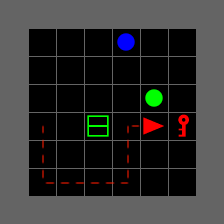
\includegraphics[width=0.49\textwidth]{figures/red_key_path}
	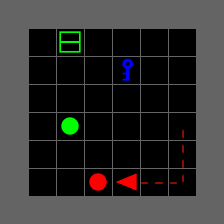
\includegraphics[width=0.49\textwidth]{figures/blue_key_path}
	\caption[An example of goal misgeneralization.]{An example of goal misgeneralization as
		a consequence of causal confusion. The intended goal is to move to the key. During training
		(left), the key is always red. The confounding goal is to move to the red object. During testing
		(right), the key can be of different colors. In other words, the red color property and the key
		object type property were spuriously correlated during training. In this case, we expect learning
		the red color property to be easier than the key object type property, which under Occam's razor
		would explain why the agent becomes causally confused and misgeneralizes at test time and navigates
		to the red ball instead.}
	\label{fig:gmg-cc-example}
\end{figure}

Accordingly, we note that GMG may therefore be addressed by tackling CC itself. In light of this, we
can distinguish three approaches. The first involves performing causal inference with the assistance
of interventions on the data so to better discover the underlying causal model. This is the main
approach of \citet{de_haan_causal_2019}. The second approach simply increases the variability of the
training data so as to reduce the likelihood of spurious correlations. This is the main approach of
\citet{langosco_goal_2022}. The final approach focuses on improving the expressiveness of the task
specification. We hypothesize that overly coarse specifications may lead to ambiguity in which task
is being requested, increasing the chance of causal confusion. We provide more detail in
Section~\ref{meth:sec:spec_causal}.

While each of these approaches have merit, we decide to focus on the third. Our motivation is
manifold. First, we expect implementations under the first approach to become increasingly more
difficult as the field shifts towards offline-learning~\citep{lange_batch_2012, levine_offline_2020,
	prudencio_survey_2022}. Secondly, while the simplicity of the second approach coupled with recent
advancements in scaling laws~\citep{kaplan_scaling_2020, hoffmann_training_2022} is promising, we
note that increasing the variability of the training data has no guarantee of de-correlating
confounding variables, especially when the spurious correlations are unknown, rendering estimating
how much and what kind of variability to work on potentially difficult for more insidious cases of
GMG~\citep{kirk_causal_2022}. We choose to focus on the approach of improving task specification not
only because we view it as an under-explored option, but more importantly because, as we will
outline in Chapter~\ref{chap:prel}, we view GMG as intrinsically tied to multi-task
learning~\citep{caruana_multitask_1997}, which itself is intrinsically tied to task specification.

\section{Grounding}\label{back:sec:grounding}

Our approach to improving task specification will focus on the notion of specifying tasks through
natural language rather than rewards.  We refer to this as \emph{language-informed sequential
	decision making (LISDM)}. Any treatment of LISDM will necessarily involve grounding, i.e. ensuring
that the language used to specify tasks is mapped to representations that can be correctly
interpreted by the agent.

More specifically, the \emph{symbol grounding problem} is the problem of ensuring that the meaning
of abstract symbols (e.g.~words) is anchored to more than the symbols
themselves~\citep{harnad_symbol_1990}. That is, symbols, on their own, are meaningless. They only
acquire meaning when they are grounded to some external referent~\citep{bender_climbing_2020} or
relation~\citep{piantadosi_meaning_2022}. For example the word ``cat'' is meaningless on its own,
but when it is grounded to the concept of a cat, it acquires meaning. The grounding problem is
a problem of communication~\citep{clark_grounding_1991}, and is therefore relevant to task
specification.

Addressing the grounding problem, at least in part, is a necessary step for an effective
implementation of LISDM. A partial treatment of the problem may be sufficient since we restrict our
focus to the context of representation learning: In certain narrowly defined LISDM scenarios, it
might be sufficient to ensure that the representations of the same concept in a few modalities are
alike~\citep{mooney_learning_2008}.

The grounding problem warrants attention primarily because the effectiveness of using language to
make decisions in a specific environment hinges on the accurate alignment of the word meanings with
that environment. Failing this, the effectiveness of language representations in guiding decisions
could be significantly compromised. Take, for instance, the case where we are endeavoring to use
language for decision-making in a restaurant setting. It becomes essential to ensure that the
representation for the term ``apple'' aligns closely with the representation of an actual apple
present in the restaurant. This is because we aim to be able to use the word ``apple'' to refer
specifically to the apple in that restaurant, rather than some other apple in a different restaurant
or another item in the same restaurant that is not an apple.


\ifSubfilesClassLoaded{%
	\bibliographystyle{\subfix{bibstyle}}
	\bibliography{\subfix{references-bibtex}}%
}{}

\end{document}
